\documentclass[11pt, oneside]{article}   	% use "amsart" instead of "article" for AMSLaTeX format
\usepackage{geometry}                		% See geometry.pdf to learn the layout options. There are lots.
\geometry{a4paper}                   		% ... or a4paper or a5paper or ...letterpaper 
%\geometry{landscape}                		% Activate for rotated page geometry
%\usepackage[parfill]{parskip}    		% Activate to begin paragraphs with an empty line rather than an indent
\usepackage{graphicx}				% Use pdf, png, jpg, or eps§ with pdflatex; use eps in DVI mode
								% TeX will automatically convert eps --> pdf in pdflatex		
\usepackage{amssymb}
\DeclareGraphicsExtensions{.pdf,.png,.jpg}
\graphicspath{ {images/} }

\usepackage{hyperref}
\usepackage{subcaption}
\usepackage{amsmath}
\usepackage{framed}
\usepackage{tabulary}
\usepackage{hyperref}


\title{Connecting Nutrition, Health and Environment }
\author{Wiktor Jurkowski, Perla Troncoso Rey, Earlham Institute}
\date{25 - 26 January 2017}	 % Activate to display a given date or no date

\begin{document}
\maketitle

\tableofcontents

\listoffigures
\listoftables


\section{Introduction}

In this practice, we will look at how to explore  gene expression data (which could be extracted from microarray or RNA sequencing data). In the first part of this practical session we will see general techniques to explore the patterns or structure of the data using Principal Component Analysis, PCA, and Hierarchical Clustering. We will then look into compiling an interaction network using an online resource and how to visualise the network using Cytoscape \cite{Shannon2003} \cite{Smoot2011}.

In the second part, we will look at ways to rank genes (and/or metabolites) using approaches based on logistic regression. We will then perform pathway analysis using those rankings.

We will use a publicly available data from a study on fatty liver disease of obese and lean human subjects \cite{Wruck2015}.



\part{Part I}

\subsection{Exploring the expression data}

One could obtain gene expression from microarrays or RNA sequencing data. It is not within the scope of this session to look at the details of obtaining quantifying the expression of genes from microarrays or RNA sequencing data but instead we will start our analysis assuming that expression data has been quantified.
The gene expression data is normally stored in tabular file, representing a matrix where the columns are the samples or experiments, and the rows represent the genes. 

Example of expression data is shown in \autoref{fig:ExpressionData}. The table shows the expression of six genes in four different experiments or samples. This is, gene A has expression of 0.1 for sample 1, 0.8 for sample 2, 0.3 for sample 3, and so forth. 

\begin{figure}[!h]
	\centering
	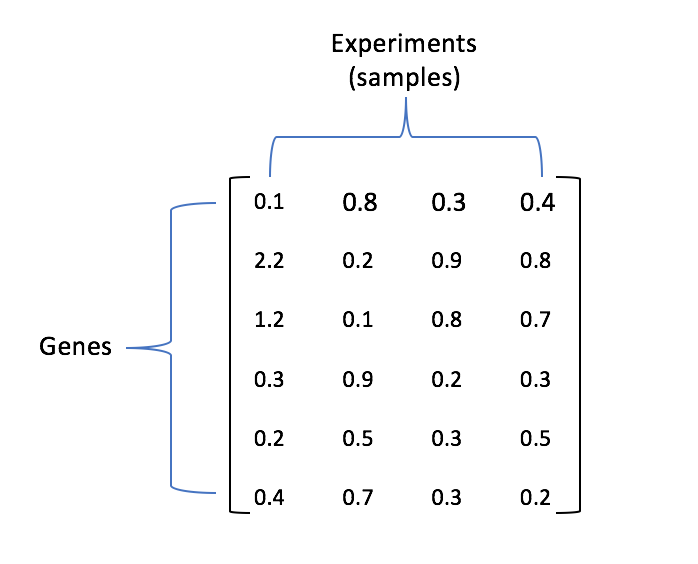
\includegraphics[width=0.7\textwidth]{example_expression_data}
	\caption{Example of expression data with samples across the columns and individual genes down the rows.}
	\label{fig:ExpressionData}
\end{figure}


Expression data can be obtained using different algorithms. One of the most well know are TopHat and Cufflinks protocol for the analysis of RNA sequencing data, which includes quantification of gene expression. \autoref{tab:ExpressionCufflinks} shows an example of the output provided by cufflinks with the estimated gene-level expression values. Cufflinks uses the notation ``XLOC\_{\it numeric\_sequence}'' to identify a gene.


\begin{table}[h]
    \centering
    \caption{Example of the output provided by cufflinks for the quantification of gene expression from RNA sequencing data.}
    \begin{tabular}{c|c|c|c|c|c|c|c|c}
    tracking\_id & sample1 & sample2 & sample3 & sample4 & sample5 & sample6 & sample7 & sample8 \\
    \hline
    XLOC\_000001 & 35.1077 & 50.9662 & 78.7724 & 35.4736 & 69.6067 & 63.9241 & 57.7967 & 61.4227 \\
    XLOC\_000002 & 49.7359 & 64.6178 & 46.8884 & 74.617 & 66.0371 & 42.9654 & 645.65 & 64.8351 \\
    XLOC\_000003 & 0 & 0 & 0.937767 & 0 & 0 & 0 & 0 & 0\\
    XLOC\_000004 & 89.7196 & 85.5504 & 185.678 & 74.617 & 142.783 & 168.718 & 172.63 & 167.206 \\
    XLOC\_000005 & 12.6778 & 39.1347 & 158.483 & 22.0181 & 28.5566 & 45.0613 & 15.9701 & 50.0481 \\
    XLOC\_000006 & 10.7273 & 9.1011 & 10.3154 & 13.4555 & 7.13915 & 6.28762 & 7.60483 & 12.512 \\
    XLOC\_000007 & 0 & 0 & 0.937767 & 0 & 0 & 0 & 0 & 0 \\
    XLOC\_000008 & 55.5871 & 37.3145 & 86.2746 & 66.0544 & 66.9295 & 53.4448 & 54.7548 & 75.0722 \\
    XLOC\_000009 & 37.0581 & 16.382 & 24.3819 & 24.4646 & 38.3729 & 15.7191 & 24.3355 & 50.0481 \\
    XLOC\_000010 & 812.352 & 483.269 & 696.761 & 748.616 & 1094.97 & 521.873 & 675.309 & 741.622 \\
    XLOC\_000011 & 0 & 0 & 0 & 0 & 0 & 1.04657 & 0.760483 & 1.13746\\
    \hline
    \label{tab:ExpressionCufflinks}
    \end{tabular}
\end{table}




\subsubsection{Principal Component Analysis}

Principal Component Analysis, commonly known as PCA, is a mathematical technique that is used to explore data, specially high-dimensional data, to extract the most important trends in the data.

When thinking of gene expression data, high dimensionality comes from the large number of dimensions of the data. This is, the result of each experiment can be thought as a kind of space, where each each feature is a coordinate in the space. There are typically thousands of genes (dimensions) and the structure of pattern in the data extends to all the dimensions. 


\paragraph{How PCA works}
\paragraph{}

The mean represents the average of the values in the data:

\begin{equation}
   \bar{{\bf X}} = \frac{1}{n} \sum_{i=1}^{n} x_i 
\end{equation}

The variance provides the the spread of the data:

\begin{equation}
   \text{Var} ({\bf X}) = \sigma^2  = \frac{1}{n-1} \sum_{i=1}^{n} ( x_i -  \bar{{\bf X}})^2
\end{equation}


For example, figure \ref{fig:MeanVariance} shows two distributions with the same mean but different variance. This means that the data points are at the same location but with a different strength. Thus, the third statistic we'll need is the covariance.

\begin{figure}[!h]
	\centering
	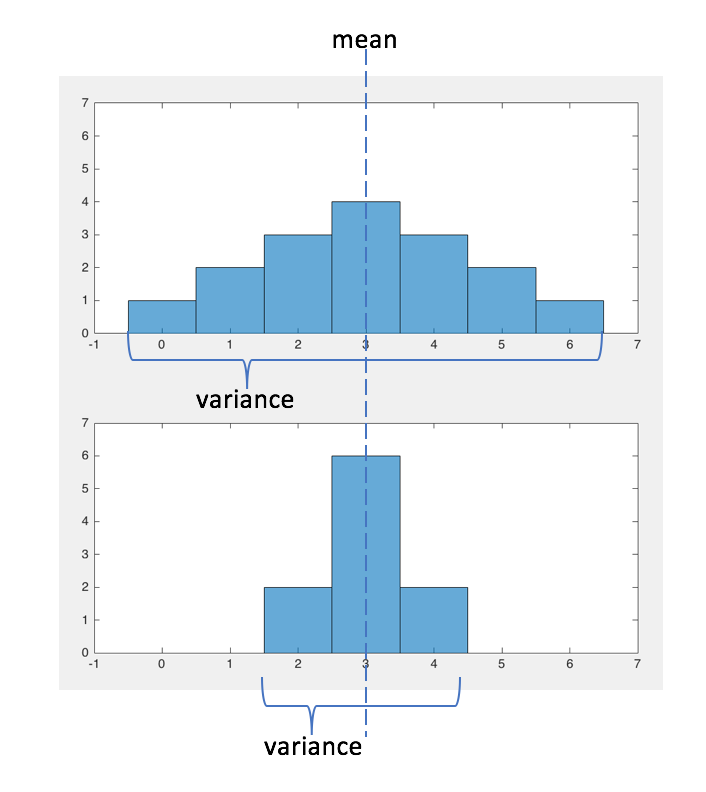
\includegraphics[width=0.7\textwidth]{same-mean_different-variance}
	\caption{Two distributions with the same mean but different variance.}
	\label{fig:MeanVariance}
\end{figure}


The covariance represents the degree of co-dependence of two variables, i.e., it measures the co-dependency of two variables, given by:

\begin{equation}
   \text{Cov} ({\bf X}, {\bf Y}) = \frac{1}{n-1} \sum_{i=1}^{n} (x_i - \bar{ {\bf X}}) (y_i - \bar{ {\bf Y}})
\end{equation}

Increases with increasing co-dependency and variance. Just as the variance measures the degree to which a set of data varies, the co-variance is a measure of the way two sets of data vary together.

\begin{equation}
   \text{Cov} ({\bf X}, {\bf X}) = \text{Var}({\bf X})
\end{equation}

The covariance also increases in magnitude as the variance of each of the two datasets increases.
Correlation values can be negative or positive, indicating whether the values of two variables increase or decrease together. Figure \ref{fig:examples-correlation} shows some examples of correlation.

\begin{figure}[!h]
	\centering
	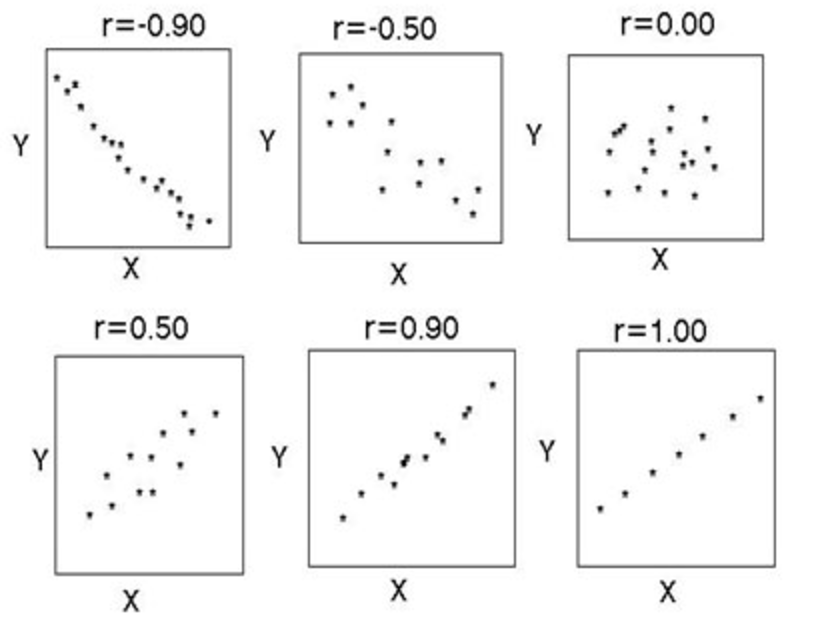
\includegraphics[width=0.7\textwidth]{examples-correlation}
	\caption{Examples of correlation}
	\label{fig:examples-correlation}
\end{figure}



\paragraph{Coordinate transformations}
\paragraph{}

In a two dimensional space described by coordinates, a point in space is described by X and Y such that ${\bf v} = [x_1, y_1]$. For example, the vector $v_1 = [1 ~2]^T$ represents a point in the 2 dimensional space as shown in Figure \ref{fig:CoordinateTransform} (a).
An alternative coordinate system described by the coordinates $\text{X}^\prime$ and $\text{Y}^\prime$, has a different column vector describing the same point ${\bf v^\prime} = [x_1^\prime, y_1^\prime]$, shown in Figure \ref{fig:CoordinateTransform} (b).

The two coordinate systems are $T{\bf v} = {\bf v}^\prime$, related to the orthogonal transform matrix $T$. An orthogonal matrix is the kind of matrix which performs rotated-axis coordinate transforms. Thus, we can make a new coordinate system by using a transformation matrix T, which relates the two coordinates vectors by matrix multiplication. There are many types of transformations but we are particularly interested in transformations which rotate the coordinate axis. These are performed by matrices which have the property called orthogonality.

\begin{figure}[!h]
	\centering
	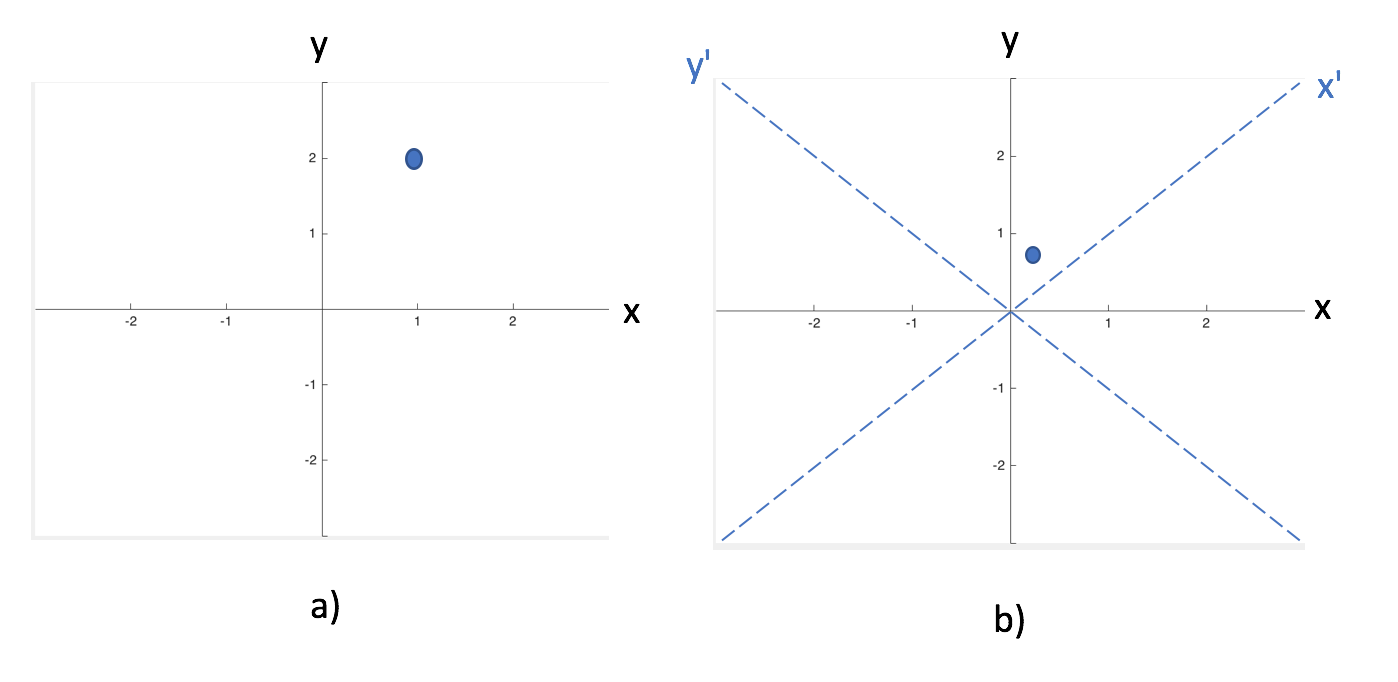
\includegraphics[width=0.7\textwidth]{example-coordinate-transform}
	\caption{Example of a coordinate transform}
	\label{fig:CoordinateTransform}
\end{figure}



\paragraph{Eigenvalues and Eigenvectors}
\paragraph{}

When a transformation matrix maps a vector to a multiple of itself, then the vector is called an Eigenvector. The amount by which the vector is multiplied (stretched) is the associated Eigenvalue:

\begin{equation}
T x = \lambda x
\end{equation} 

\noindent where $\lambda$ are the Eigenvalues and $x$ are the Eigenvectors. 

In general terms, PCA uses covariance to encode the structure in the data and then eigenvectors to devise a new set of coordinates that best reveals the structure by finding the appropriate set of directions. One result from linear algebra is that if the eigenvectors are placed next to each other to construct an orthogonal matrix that performs a coordinate transformation. It is important to mention that Eigenvectors are placed in descending order of their corresponding eigenvalue to ensure that the first components encode most of the variance in the data.
The transpose of this matrix of Eigenvectos is an orthogonal matrix which performs a rotated-axis coordinate transformation. We can transform our data matrix, $D$, to the new coordinates, $D_{PCA}$:  

\[
   D_{PCA} = W^T D
\]


For example: 

\[ \text{The matrix: }
%
   \left(
      \begin{tabular}{cc}
      1 & 3 \\ 
      2 & 2
      \end{tabular}
   \right)
   %
   \text{has eigenvalues 4 and -1}
   \text{ and the eigenvectors}
   \left( \begin{array}{c}
      1 \\ 
      1
      \end{array}
   \right)
   \text{and} 
   \left( \begin{array}{c}
      3 \\ 
      -2
      \end{array}
   \right)
\]


such that

\[ \left( \begin{array}{cc}
      1 & 3\\ 
      2 & 2
      \end{array} \right)
%
   \left( \begin{array}{c}
      1 \\ 
      1
      \end{array} \right)
%
   = 4
   \left( \begin{array}{c}
   1\\
   1
   \end{array} \right)
\text{~~~and~~~}
   \left( \begin{array}{cc}
   1 & 3\\
   2 & 2
   \end{array} \right)
%
   \left( \begin{array}{c}
   3\\
   -2
   \end{array} \right)
%
   =-1
   \left( \begin{array}{c}
   3\\
   -2
   \end{array} \right)
\]

The orthogonal matrix using these Eigenvector is: 

\[ 
  W^T = 
   \left[ \begin{array}{cc}
      1 & 1 \\ 
      3 & -2      
   \end{array} \right]
\]



% Here we start with some hands-on exercises

% Example 1
\subsubsection{Exercise: PCA for the expression of two genes}
\paragraph{}

We will use R and the package stats to perform PCA. We will use an example data which represents several measurements of the expression of two genes, $x$ and $y$, with the following values:

\begin{center}
\begin{tabular}{c|c}
   x & y \\
   \hline
   2.5 & 2.4\\
   0.5 & 0.7\\
   2.2 & 2.9\\
   1.9 & 2.2\\
   3.1 & 3.0\\
   2.3 & 2.7\\
   2.0 & 1.6\\
   1.0 & 1.1\\
   1.5 & 1.6\\
   1.1 & 0.9\\
   \hline
\end{tabular}
\end{center}
   

We start by create a matrix of points in 2-d space (gene expression data) by using the following syntax:

%% create a matrix with the data from two genes
% script
% x <- c(2.5, 0.5, 2.2, 1.9, 3.1, 2.3, 2.0, 1.0, 1.5, 1.1)
% y <- c(2.4, 0.7, 2.9, 2.2, 3.0, 2.7, 1.6, 1.1, 1.6, 0.9)
% class <- c('control', 'control', 'control', 'control', 'control',
%  'case', 'case', 'case', 'case', 'case')
% ExpData <- data.frame(x = x, y = y, class = class)
	
\begin{framed}
\begin{verbatim}
   #n number of samples
   name_gene_1 <- c(values_in_sample1, ..., _value_in_sampleN) 
   #m number of genes
   name_gene_2 <- c(gene_1, gene_2, ..., gene_m)    
   samples <- c(sample1, ..., sampleN)
   # expression matrix
   Exp <- data.frame(gene1 = name_gene1, ..., geneM = name_geneM)	
\end{verbatim}
\end{framed}


Then, we plot these two genes (see figure \ref{fig:PlotTwoGenes}) using the command: 

\begin{framed}
\begin{verbatim}
   plot(x, y)
\end{verbatim}
\end{framed}


\noindent Trends are already apparent because data is simple but this is not usually the case. We then perform an statistical analysis using Principal Component Analysis. Before starting with PCA, it is best to first have centered the data with mean zero. This is, calculate the mean of each of the two variables and substracted to obtain centered data (shown in figure \ref{fig:PlotTwoGenesCentered}). 


%Plot data and data centered
\begin{figure}[!h]
	\centering
	\begin{subfigure}{.45\textwidth}
		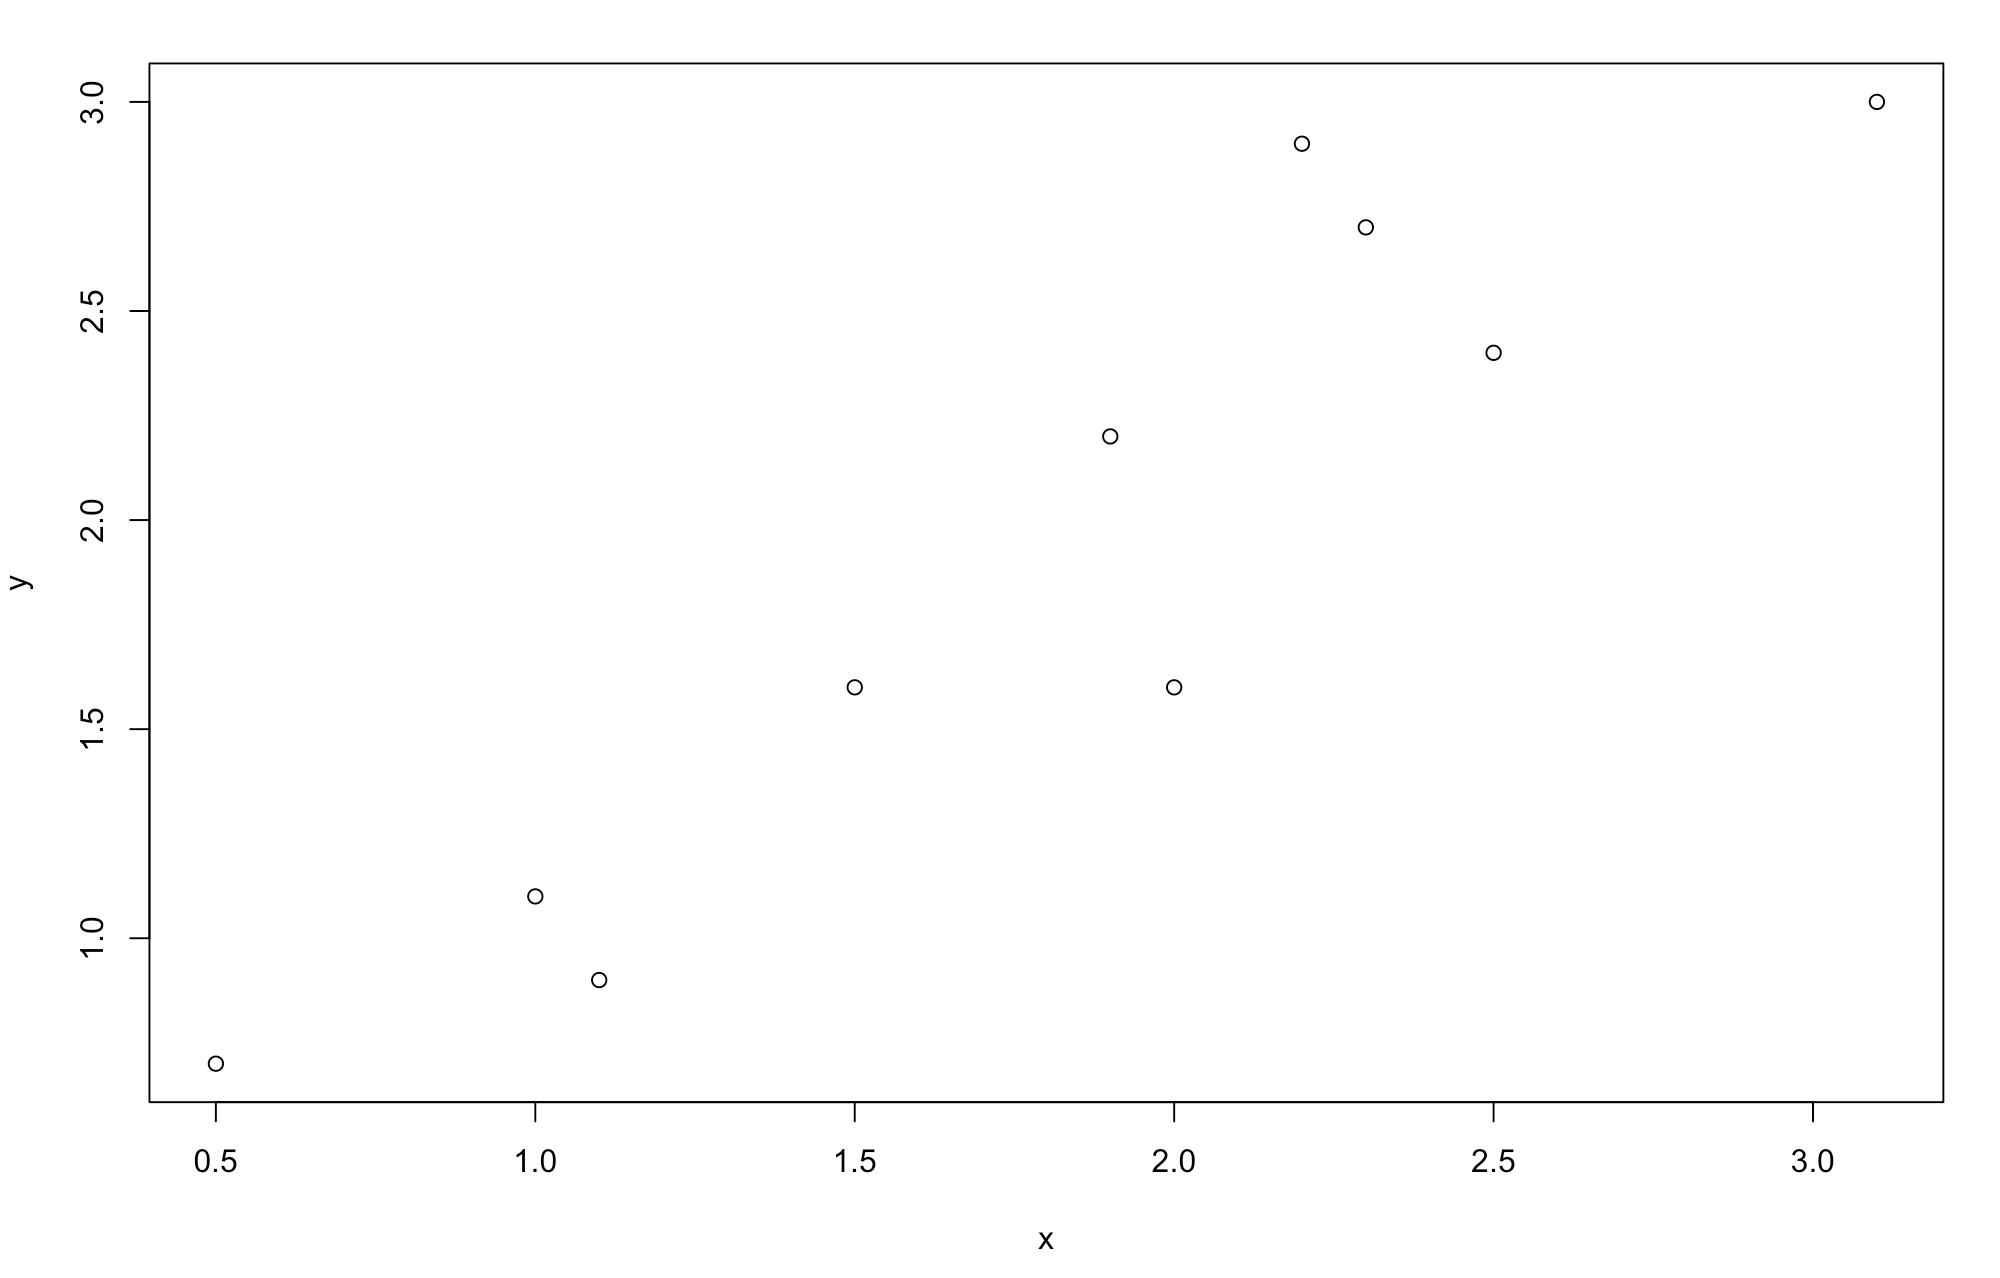
\includegraphics[width=\textwidth]{example1-plot-two-genes}
		\caption{}
		\label{fig:PlotTwoGenes}
	\end{subfigure}
	\begin{subfigure}{0.45\textwidth}
		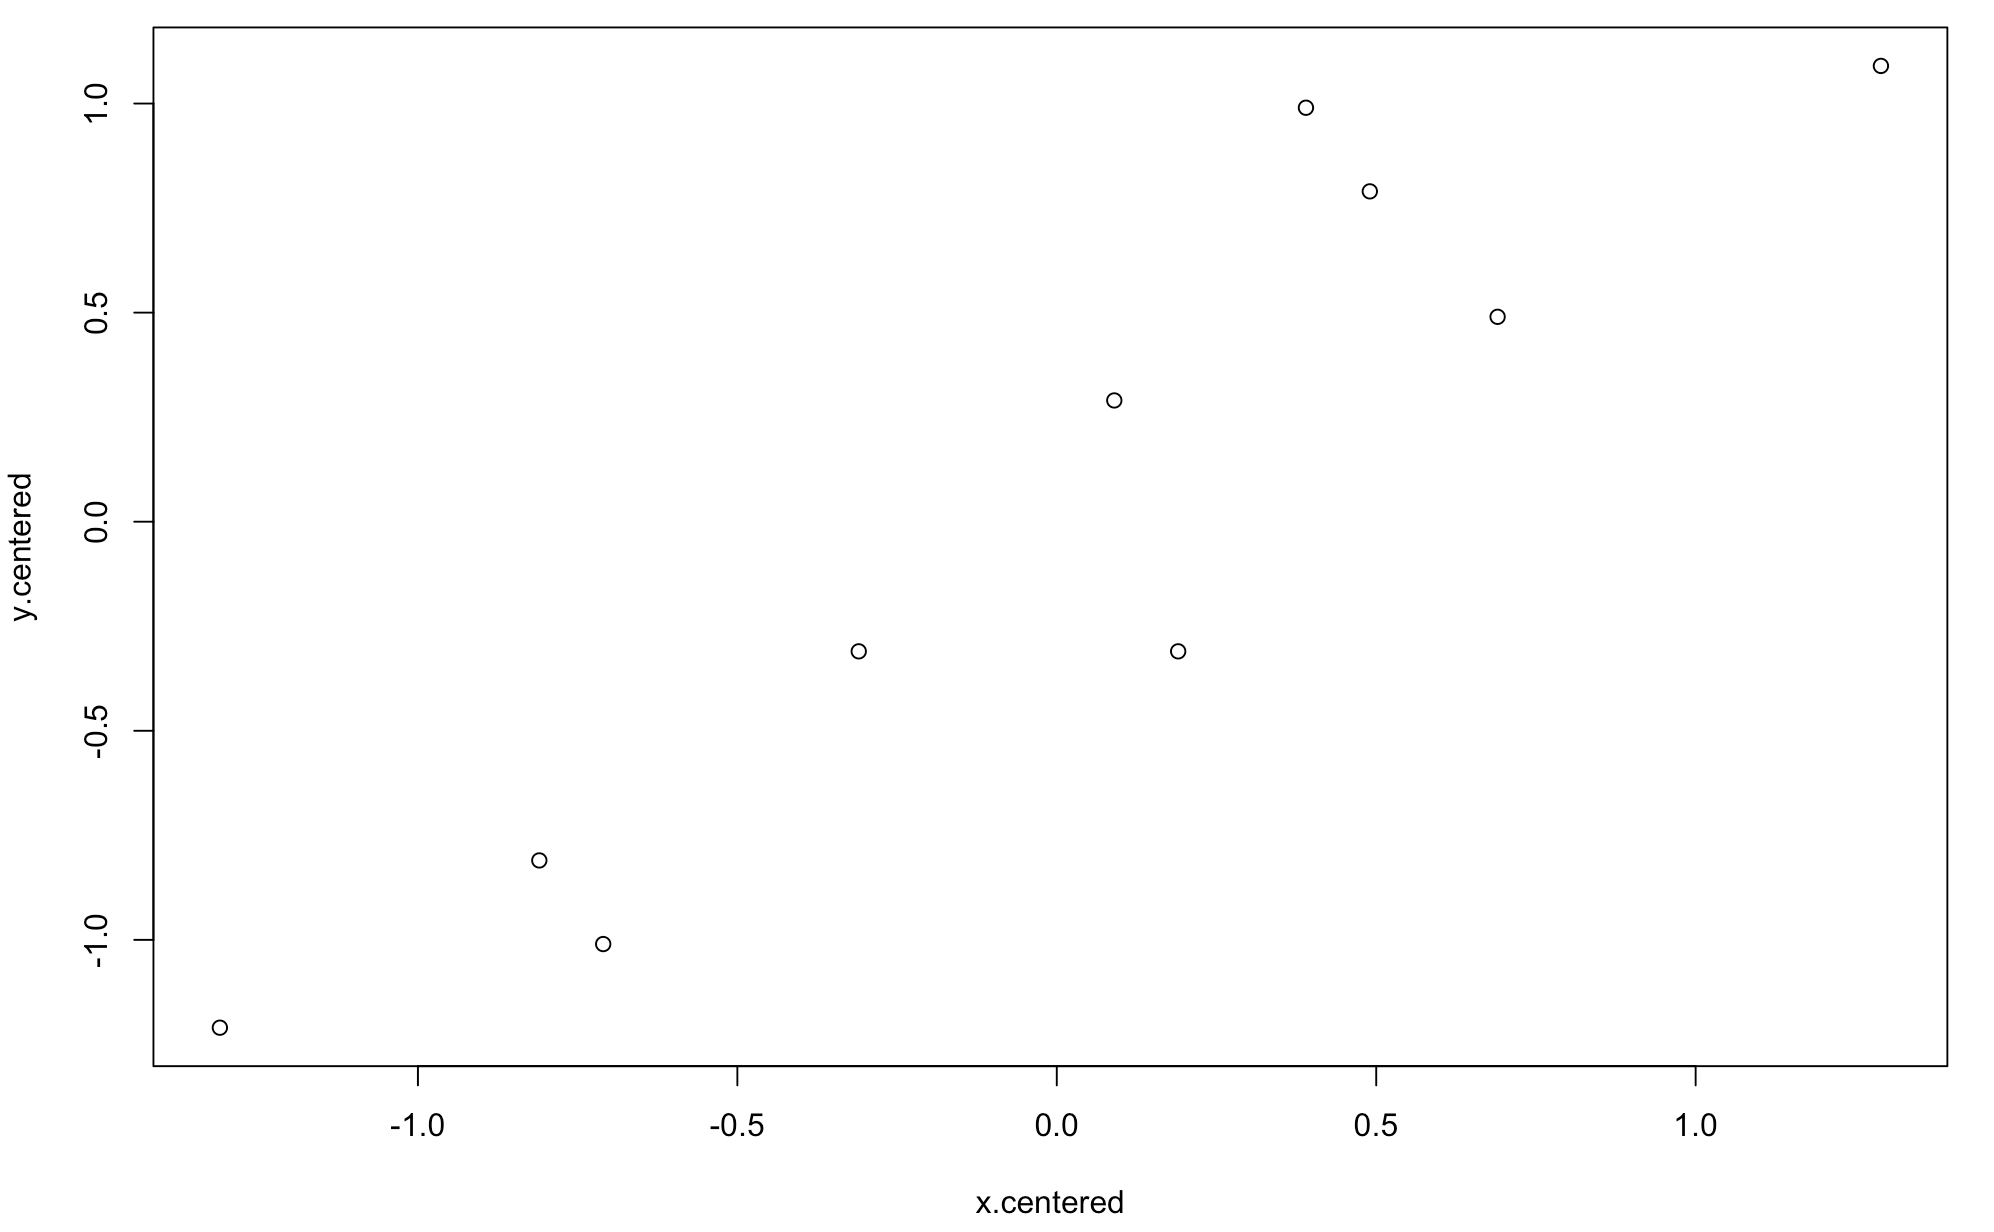
\includegraphics[width=\textwidth]{example1-plot-two-genes-centered}
		\caption{}
		\label{fig:PlotTwoGenesCentered}
	\end{subfigure}
	\begin{subfigure}{0.45\textwidth}
		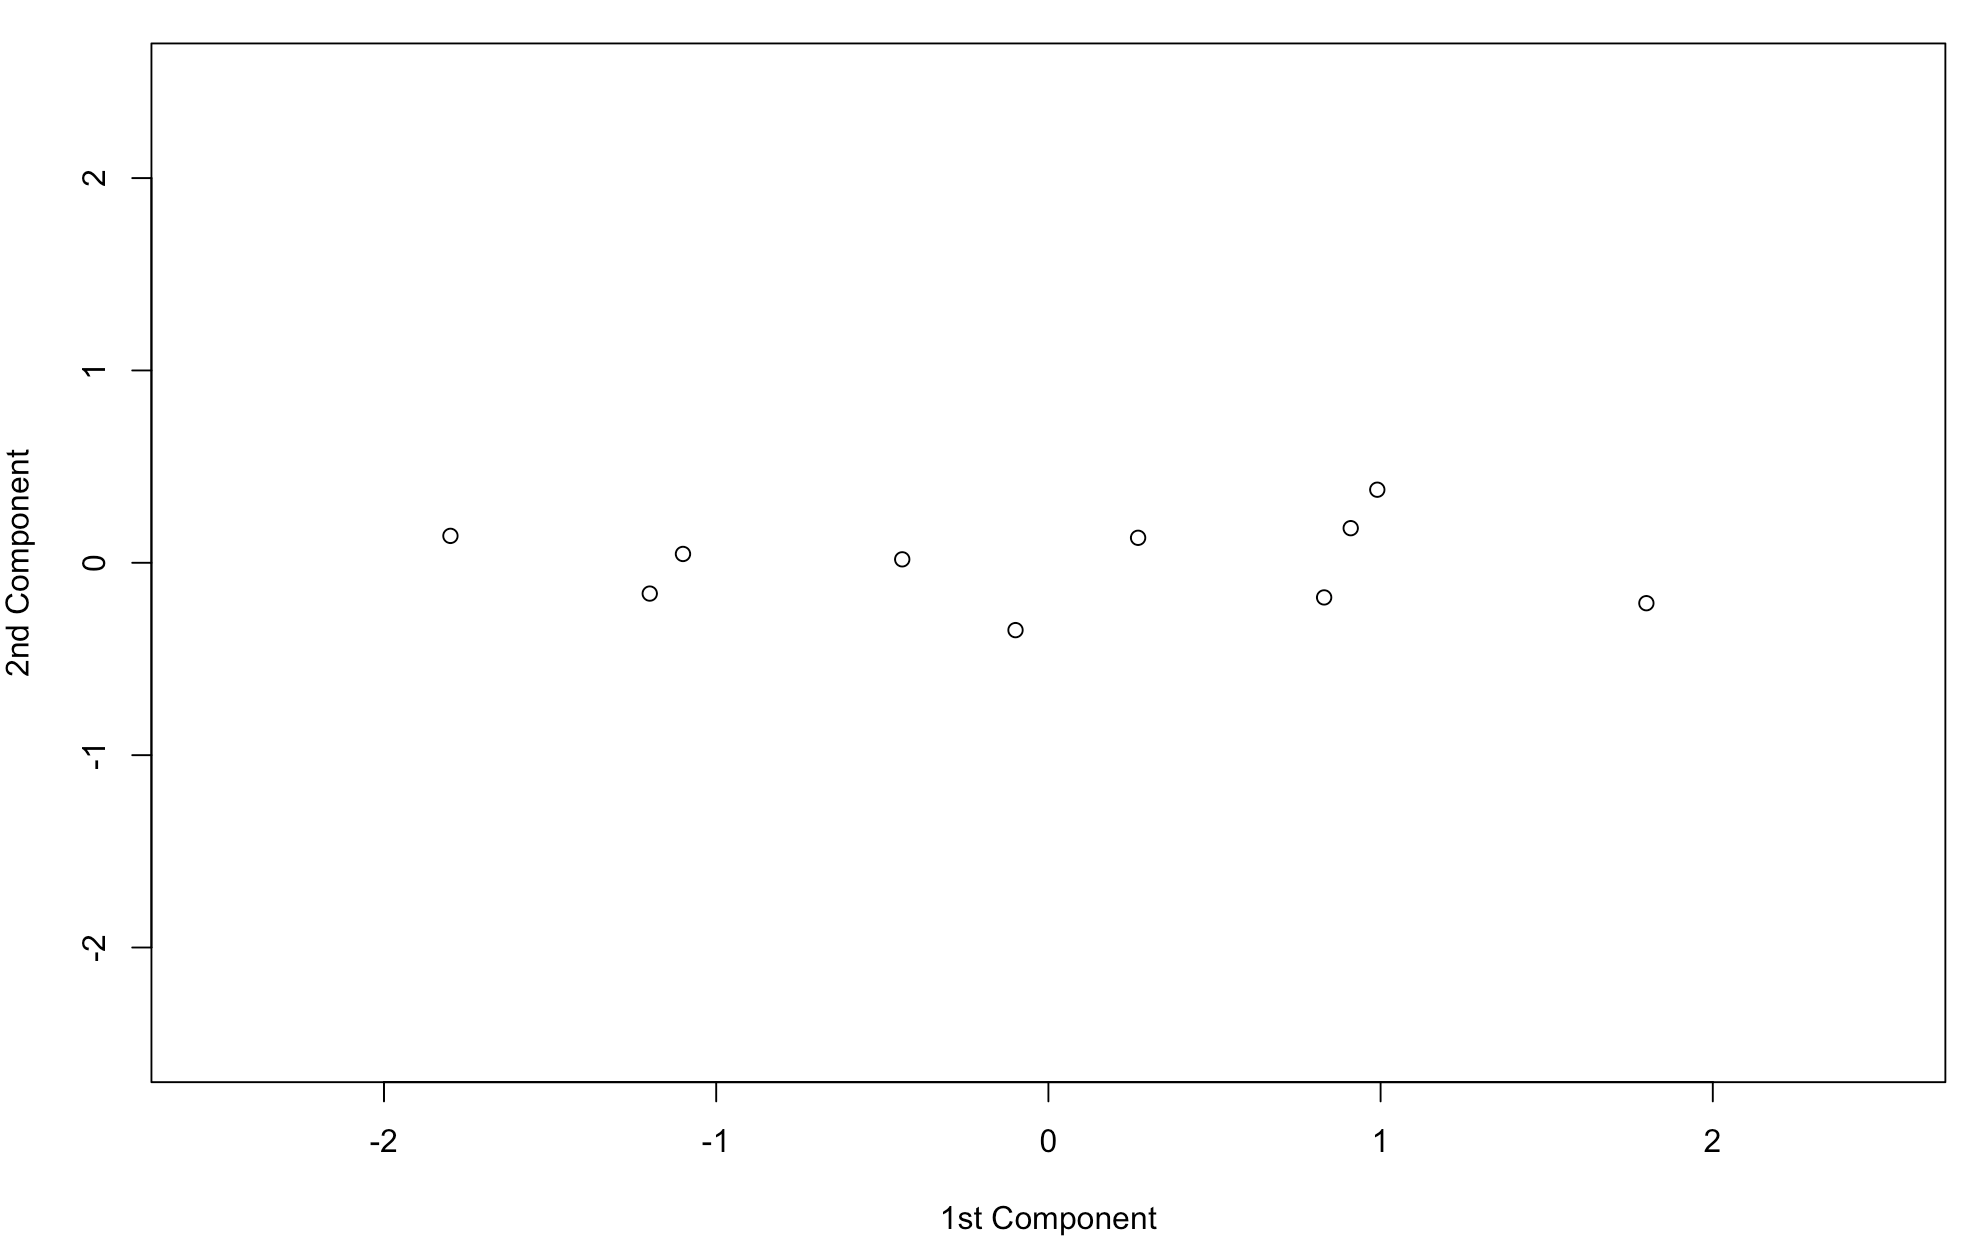
\includegraphics[width=\textwidth]{example1_plot_2PC}
		\caption{}
		\label{fig:PlotTwoGenesNewCoordiantes}
	\end{subfigure}
	\caption{Plot: in (a) shows the expression of two genes, (b) the expression of the same two genes after centering the data (expression has zero mean),  (c) gene expression is plot in the new coordiantes (PCA)}
	\label{fig:PlotData}
\end{figure}


Now, let us calculate the covariance matrix. Covariance matrix for two variables:

\[ \left[ \begin{array}{cc}
      $Cov(x,x)$ & $Cov(x,y)$\\ 
      $Cov(y,x)$ & $Cov(y,y)$
      \end{array} \right]
\]

\noindent and Covariance matrix for our data:
\[
   \left[ \begin{array}{cc}
      0.016 & 0.615 \\ 
      0.615 & 0.716
      \end{array} \right]
\]

The Eigenvalues of this matrix are:  1.284 and 0.0490. Eigenvalues gives the relative variance of the data in the direction defined by the Eigenvectors. From the values we can inferred that most variation is in one direction. To calculate the Eigenvalues in R use type:

\begin{framed}
\begin{verbatim}
	eigen(covariance_matrix)
\end{verbatim}
\end{framed}

The corresponding eigenvector are then placed in a matrix in descending order of eigenvalue:

\[
   \left[ \begin{array}{cc}
	0.6778734 & $-0.7351787$ \\
	0.7351787 & 0.6778734
      \end{array} \right]
\]

The transpose of this Eigenvectos will perform the coordinate transformation:

\[
   W^T = 
   \left[ \begin{array}{cc}
	0.6778734 & 0.7351787 \\
	$-0.7351787$ & 0.6778734
      \end{array} \right]
\]

\noindent This is an orthogonal matrix which performs a rotated-axis coordinate transformation.
We can transform our data matrix so that the data is represented in the new coordinates:  

\[
   D_{PCA} = W^T D
\]

\noindent which in our example is:

\[
   D_{PCA} = 
   \left[ \begin{array}{cc}
	0.6778734 & 0.7351787 \\
	$-0.7351787$ & 0.6778734
   \end{array} \right]
   %
   \left[ \begin{array}{cccccccccc}
      0.69 & $-1.31$ & 0.39 & 0.09 & 1.29 & 0.49 & 0.19 & $-0.81$ & $-0.31$ & $-0.71$ \\
      0.49 & $-1.21$ & 0.99 & 0.29 & 1.09 & 0.79 & $-0.31$ & $-0.81$ & $-0.31$ & $-1.01$
   \end{array} \right]
\]

\[
   =
   %
   \left[ \begin{array}{cccccccccc}
      0.83 & $-1.8$ & 0.99 & 0.27 & 1.8 & 0.91 & $-0.099$ & $-1.1$ & $-0.44$ & $-1.2$ \\
      $-0.18$ & 0.14 & 0.38 & 0.13 & $-0.21$ & 0.18 & $-0.35$ & 0.046 & 0.018 & $-0.16$
   \end{array} \right]
\]


The we can plot our data in the new coordinates, as shown in figure \ref{fig:PlotTwoGenesNewCoordiantes}, where each coordinate is called principal component. 
The first coordinate aligns with the direction in the expression space where has the most variation. Subsequent coordinates would align with directions with descending degrees of variation. This is why we are careful to order according to the size of the eigenvalues.
Thus, PCA is capturing as much variation in the first component as possible, then the same for the second coordinate, and so on.
In the case of our data, all the meaningful variation sees to have been captured with the first coordinate, or the first principal component. Specially compared to the second component which would seem to be random scatter. So we have reduced the dimensionality of our data from two to one. In cases when dealing with thousands of genes, PCA might be able to capture most of the variation of the data in with only two or three principal components. Thus making it easier to visualise it, which is one of the main motivations of performing PCA.


\begin{figure}[!h]
	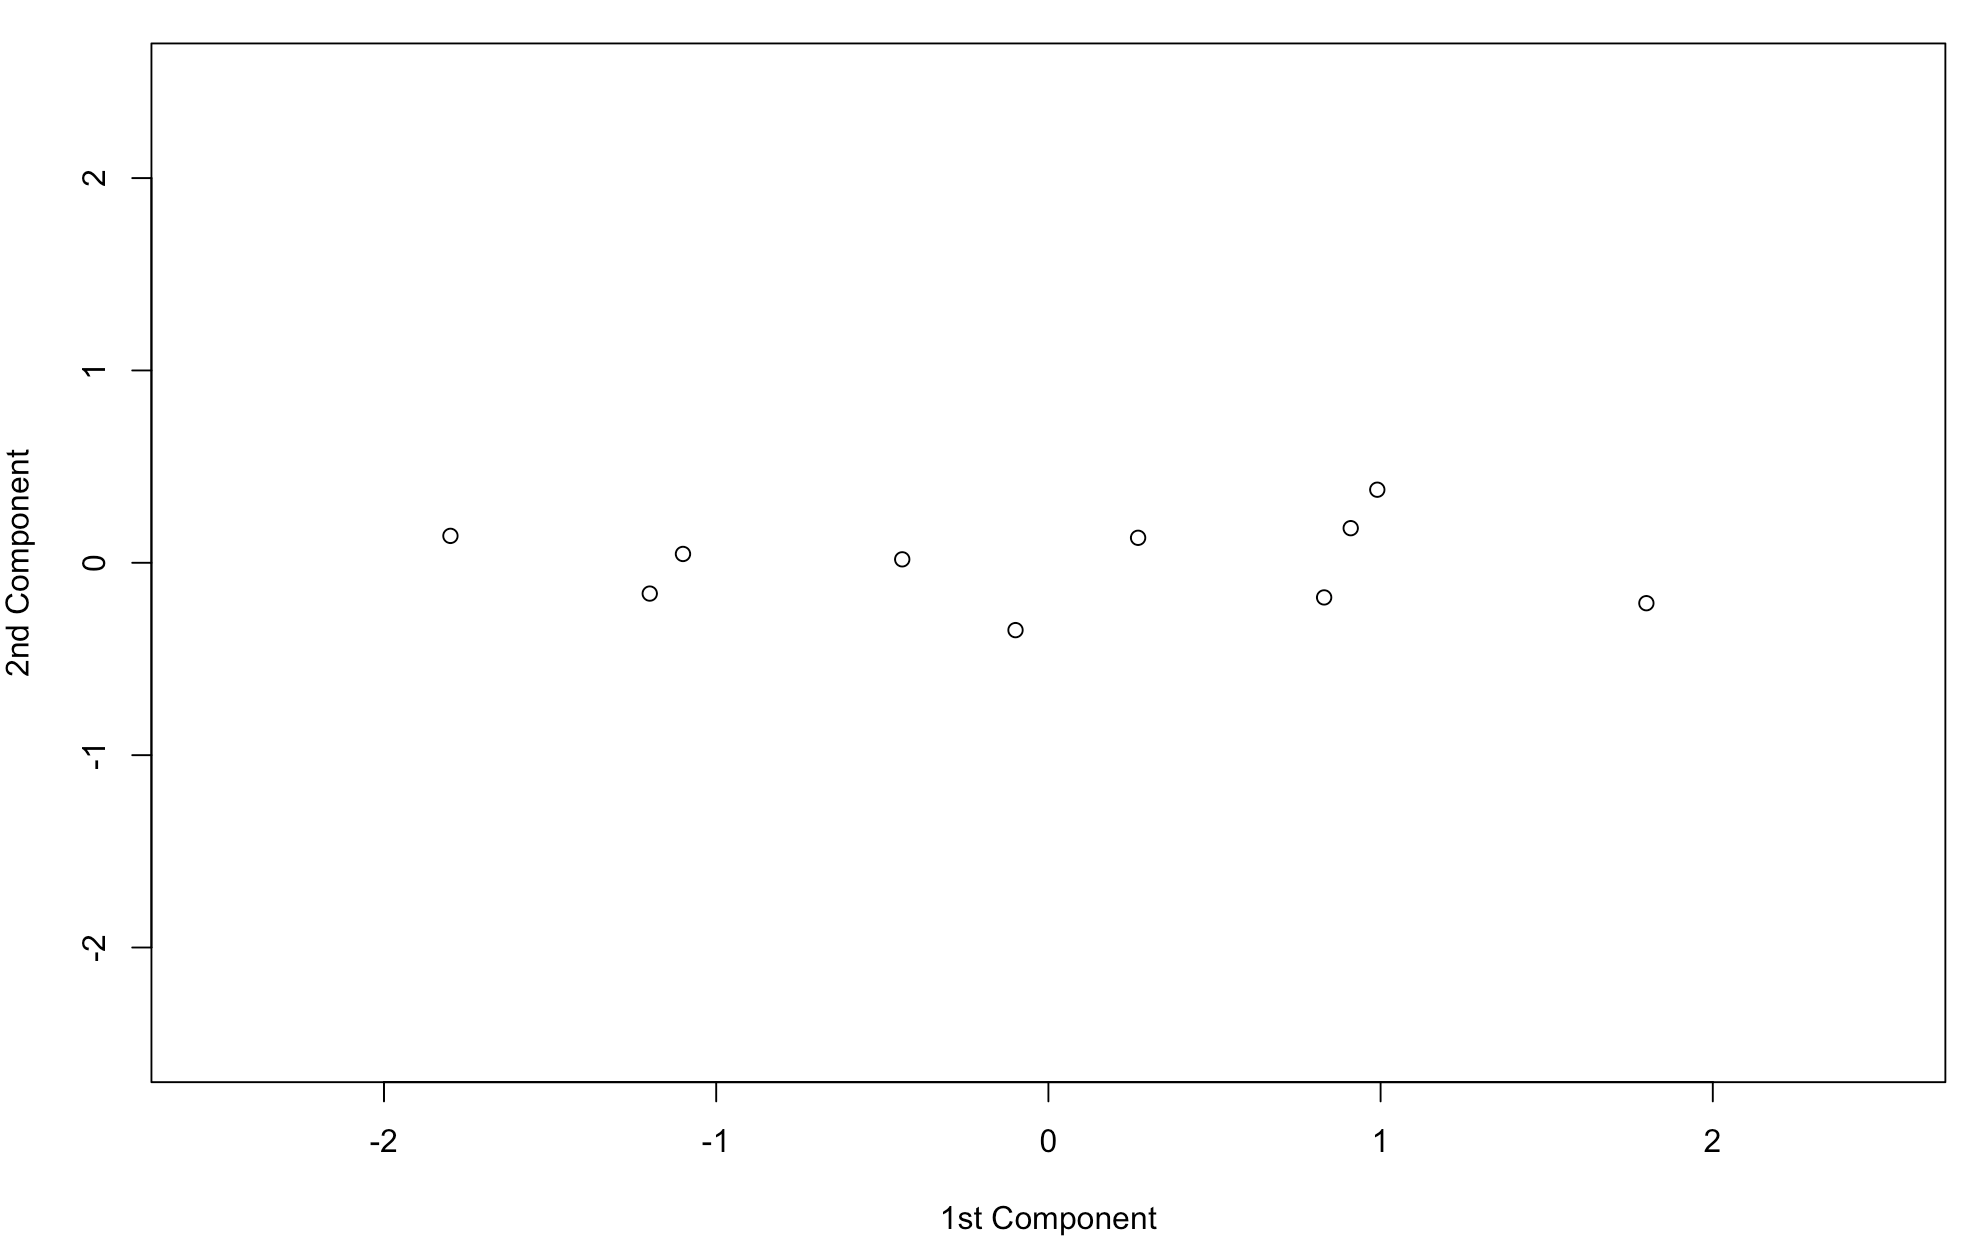
\includegraphics[width=\textwidth]{example1_plot_2PC}
	\caption{Plot of two genes in the new coordinates}
	\label{fig:PlotTwoGenesNewCoordiantes}
\end{figure}




% Example 2: loading example data from file
\subsubsection{Exercise: PCA using example data}


In this example we will use a publicly available dataset to explore expression data. We will use the stats package in R for computing PCA and will show how to visualise it using the function ggbiplot, which was implemented by Vince Q Vu \cite{Vu2016}. 


Gene expression data is usually stored in a tab delimited text file. The extension of such files could be .csv, .soft, .xls(x), etc. Use Excel, R or MATLAB to open and preview the file. It is important to mention that gene expression values must be normalised before PCA plotting.

The dataset used in this example is from a study on non-alcoholic fatty liver disease, published in 2015 by Wruck et al. \cite{Wruck2015}. The transcriptomics data was extracted from nine from patients that were recruited in the Multidisciplinary Obesity Research project at the Medical University of Graz, Austria, or at the Interdisciplinary Adipositas Center at the Kantonsspital St Gallen, Switzerland. Each sample is described in table \ref{tab:ExpressionDataWruck}) in terms of gender, age, BMI, percent of steatosis and steatosis grouping.

\begin{table}[h]
	\centering
	\caption{Details of the samples for microarray data for a study in fatty liver \cite{Wruck2015}}
	\begin{tabular}{c | c | c | c | c | c}
		\hline
		ID & gender & age & BMI & \% steatosis & steatosis grouping \\
		\hline
                H0004 & f & 54 & 47 & 10 & obese, low steatosis \\
                H0007 & f & 33 & 51 & 40 & obese, high steatosis \\
                H0008 & m & 61 & 46 & 40 & obese, high steatosis \\
                H0009 & f & 48 & 49 & 5 - 10 & obese, low steatosis \\
                H0011 & f & 58 & 45 & 70 & obese, high steatosis \\
                H0012 & f & 50 & 35 & 0 & obese, low steatosis \\
                H0018 & f & 35 & 41 & 30 - 40 & obese, high steatosis \\
                H0021 & m & 49 & 41 & 0 & no steatosis \\
                H0022 & m & 45 & 49 & 40 & obese, high steatosis
		\label{tab:ExpressionDataWruck}
	\end{tabular}
\end{table}


The gene expression matrix, gene annotation and sample annotation can be found in the following files:

\begin{itemize}
   \item {\bf gene-expression-table.txt}: gene expression table. This table is available as reference but for the simplicity we will use the following files which contain the expression data separately from the gene annotation, the names of samples, and the steatosis groups per sample.
   \item {\bf gene-expression.txt}: numerical matrix for the gene expression values, where the columns represent genes and the rows represent the samples. This is the transpose of the expression matrix because the function requires the rows of the input matrix to be observations and the columns features, which means rows to be the gene expression profiles (samples) and columns to be the genes.
   \item {\bf gene-annotation.txt}: string vector containing the gene names for the expression data
   \item {\bf samples.txt}: name of each sample
   \item {\bf groups.txt}: name of the steatosis group for each sample
\end{itemize}


Now, we can load the data into R to begin the analysis. We can either load the gene expression table by typing:

% Load data from files
\begin{framed}
\begin{verbatim}
#Expression data is saved in a tabular txt file
#The data is in a numerical matrix with no headers
	ExpData <- read.delim(FileName, header = FALSE, sep = '\t', 
		stringsAsFactors = FALSE)
	Annotation <- read.delim(FileName, header = TRUE, sep = '\t', 
		stringsAsFactors = FALSE)
	samples <- read.delim(FileName, header = TRUE, sep = '\t', 
		stringsAsFactors = FALSE)
	genes.class <- read.delim(FileName, header = TRUE, sep = '\t', 
		stringsAsFactors = FALSE)
\end{verbatim}
\end{framed}

Next, calculate the principal components using {\it prcomp} and plot the first two components. Then plot the first two components using {\it ggbiplot} \cite{Vu2016}:    

\begin{framed}
\begin{verbatim}
## Computing the principal components using prcomp
        genes.pca <- prcomp(gene_expression_data)
        
	# Plot the components using ggbiplot
        library(ggbiplot)
        
        g <- ggbiplot(genes.pca, obs.scale = 1, var.scale = 1,
                      groups = genes.class$groups, ellipse = TRUE,
                      circle = FALSE, var.axes = FALSE) +
          scale_color_discrete(name = '') +
          theme(legend.direction = 'horizontal', legend.position = 'top')
        
        print(g)
\end{verbatim}
\end{framed}


\noindent {\it ggbiplot} produces a plot which is shown in figure \ref{fig:PCAFattyLiver}.
Each dot is a gene expression from a sample in each category (group) from a patient, and is coloured by its type.
The two axis are the first two principal components and the numbers represent the percentage of variance that is captured by each component. Typically, the first three component captures the most variance, whereas following components capture only a small percentage of variance.
Dots of the same type tend to cluster together which means that samples of the same type have similar expression profiles.
The distance on the dots on each axis should not be treated equally (as each component captures a different percentage of variance). Thus, the difference on the first component should be taken into more consideration.
Furthermore, the ellipse in the figure represents the normal data ellipse for each group for the details of 68\%. 

\begin{figure}[!h]
	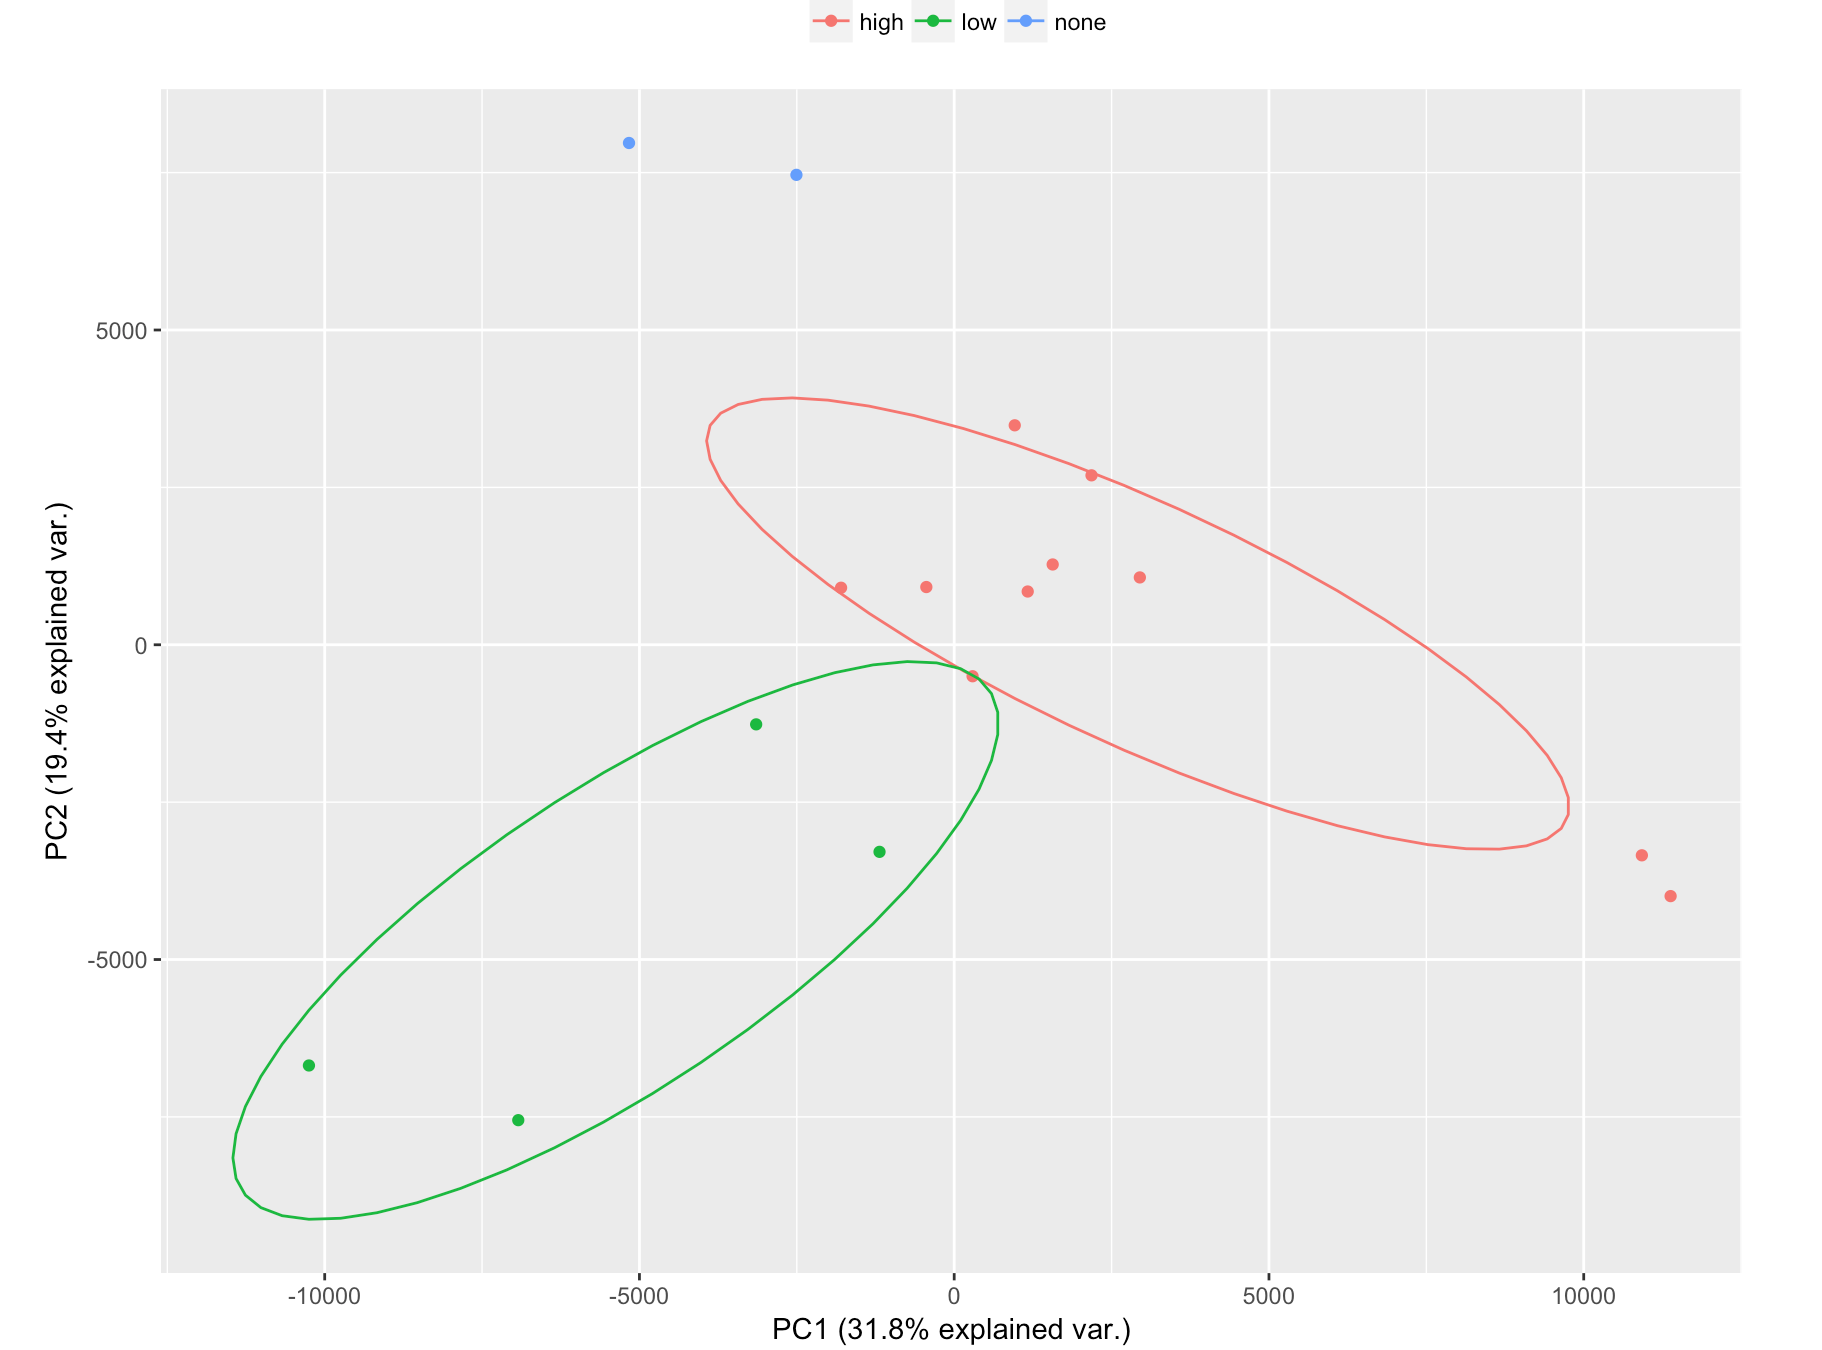
\includegraphics[width=\textwidth]{example2-first2components-fattyLiverData}
	\caption{The first two principal components for gene expression data in a study on Fatty Liver. The plot was generated using the R package ggbiplot \cite{Vu2016}}
	\label{fig:PCAFattyLiver}
\end{figure}




\paragraph{Exercise 3}
\paragraph{}

Plot the three principal components for the expression data.
Figure \ref{fig:example2-PCA-3D} shows an example of such plot.

\begin{figure}[!h]
	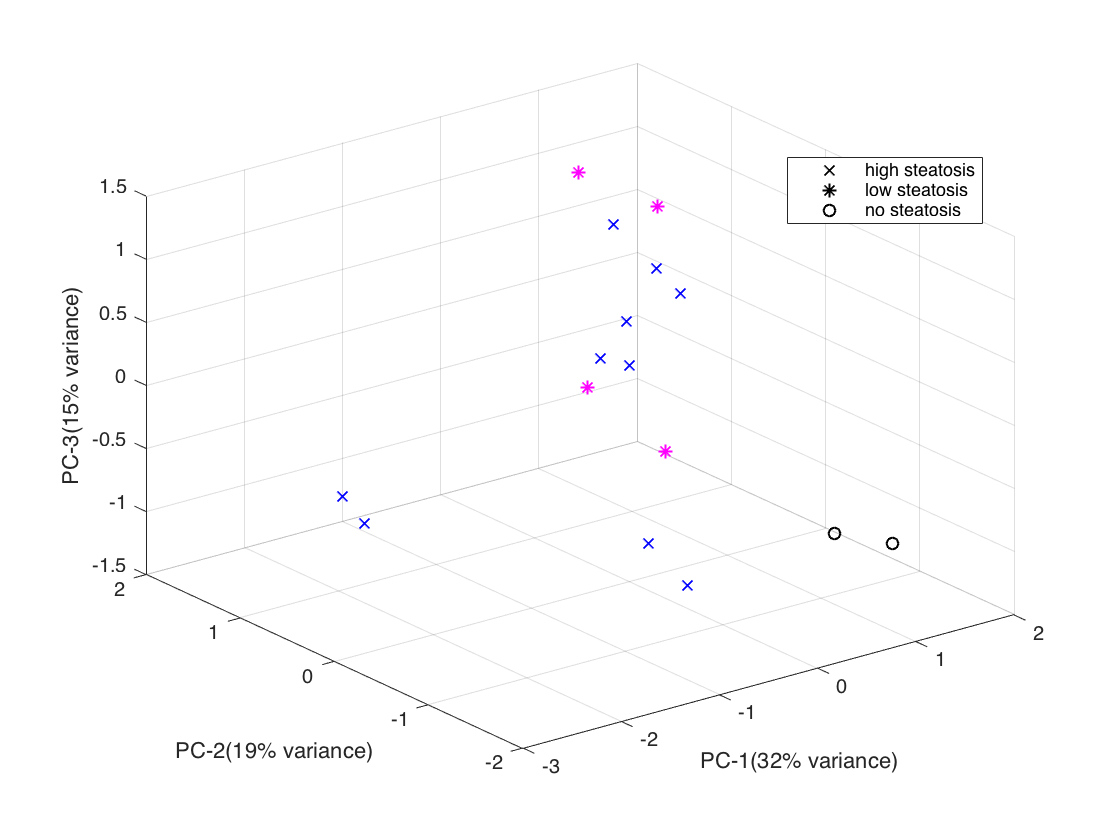
\includegraphics[width=\textwidth]{example2-PCA-3D}
	\caption{The first three principal components for gene expression data in a study on Fatty Liver \cite{Wruck2015}. Note: the plot was generated using MATLAB, can you plot the three components in R}
	\label{fig:example2-PCA-3D}
\end{figure}


\paragraph{Summary}
\paragraph{}

In summary, PCA is a method of revealing underling trends in large amounts of data. PCA reduces high dimensional data to just a few principal components which hopefully capture most of the variation of the data and allows inferring meaningful structure.

A new coordinate system is constructed by rotating the axes (each representing a gene). The first new coordinate, or first principal component, is the direction in which the data varies most, then the second component, and so on. PCA allows to select a few new variables which contain most of the variation of the data which can also be visualised.


Some of the benefits of using PCA benefits are:

\begin{itemize}

   \item A powerful tool to visualise high dimensional data 

   \item Shows quantified difference among observations

   \item Used to assess data quality and discover relationships between data points
   
   \item Some software to compute PCA is available in MATLAB and R (using package stats)

\end{itemize}





\subsubsection{Hierarchical Clustering}

Hierarchical Clustering is another way to visualise high dimensional data. 
It clusters observations by distance and builds a hierarchical structure.
It gives more detailed information of the differences among clusters, for example, what genes contributes the most to the differences between two clusters.


Hierarchical clustering uses a distance metric (typically Euclidean but could be correlation, Hamming distance, etc.) between each pair of genes to create a hierarchical tree-like structure of the data. Then it uses a linkage function to calculate the distance between clusters. For more details please see \cite{Clustergram}. 


Figure \ref{fig:hierarchical-clustering} shows an example of clustergram from gene expression data.
The clustergram is made of a heat map in the middle and dendograms in the left and top, with row and column labels on the right and bottom (depending on the number of genes and samples) and a scale bar. 
Each column is a sample expression profile, and each row represents a gene.
The colours suggests relative expression values, where red indicates high expression values and blue indicates low expression values. 
Ideally, samples of the same type will cluster together, e.g., all control samples will cluster together and all cases as well.

\begin{figure}[!h]
	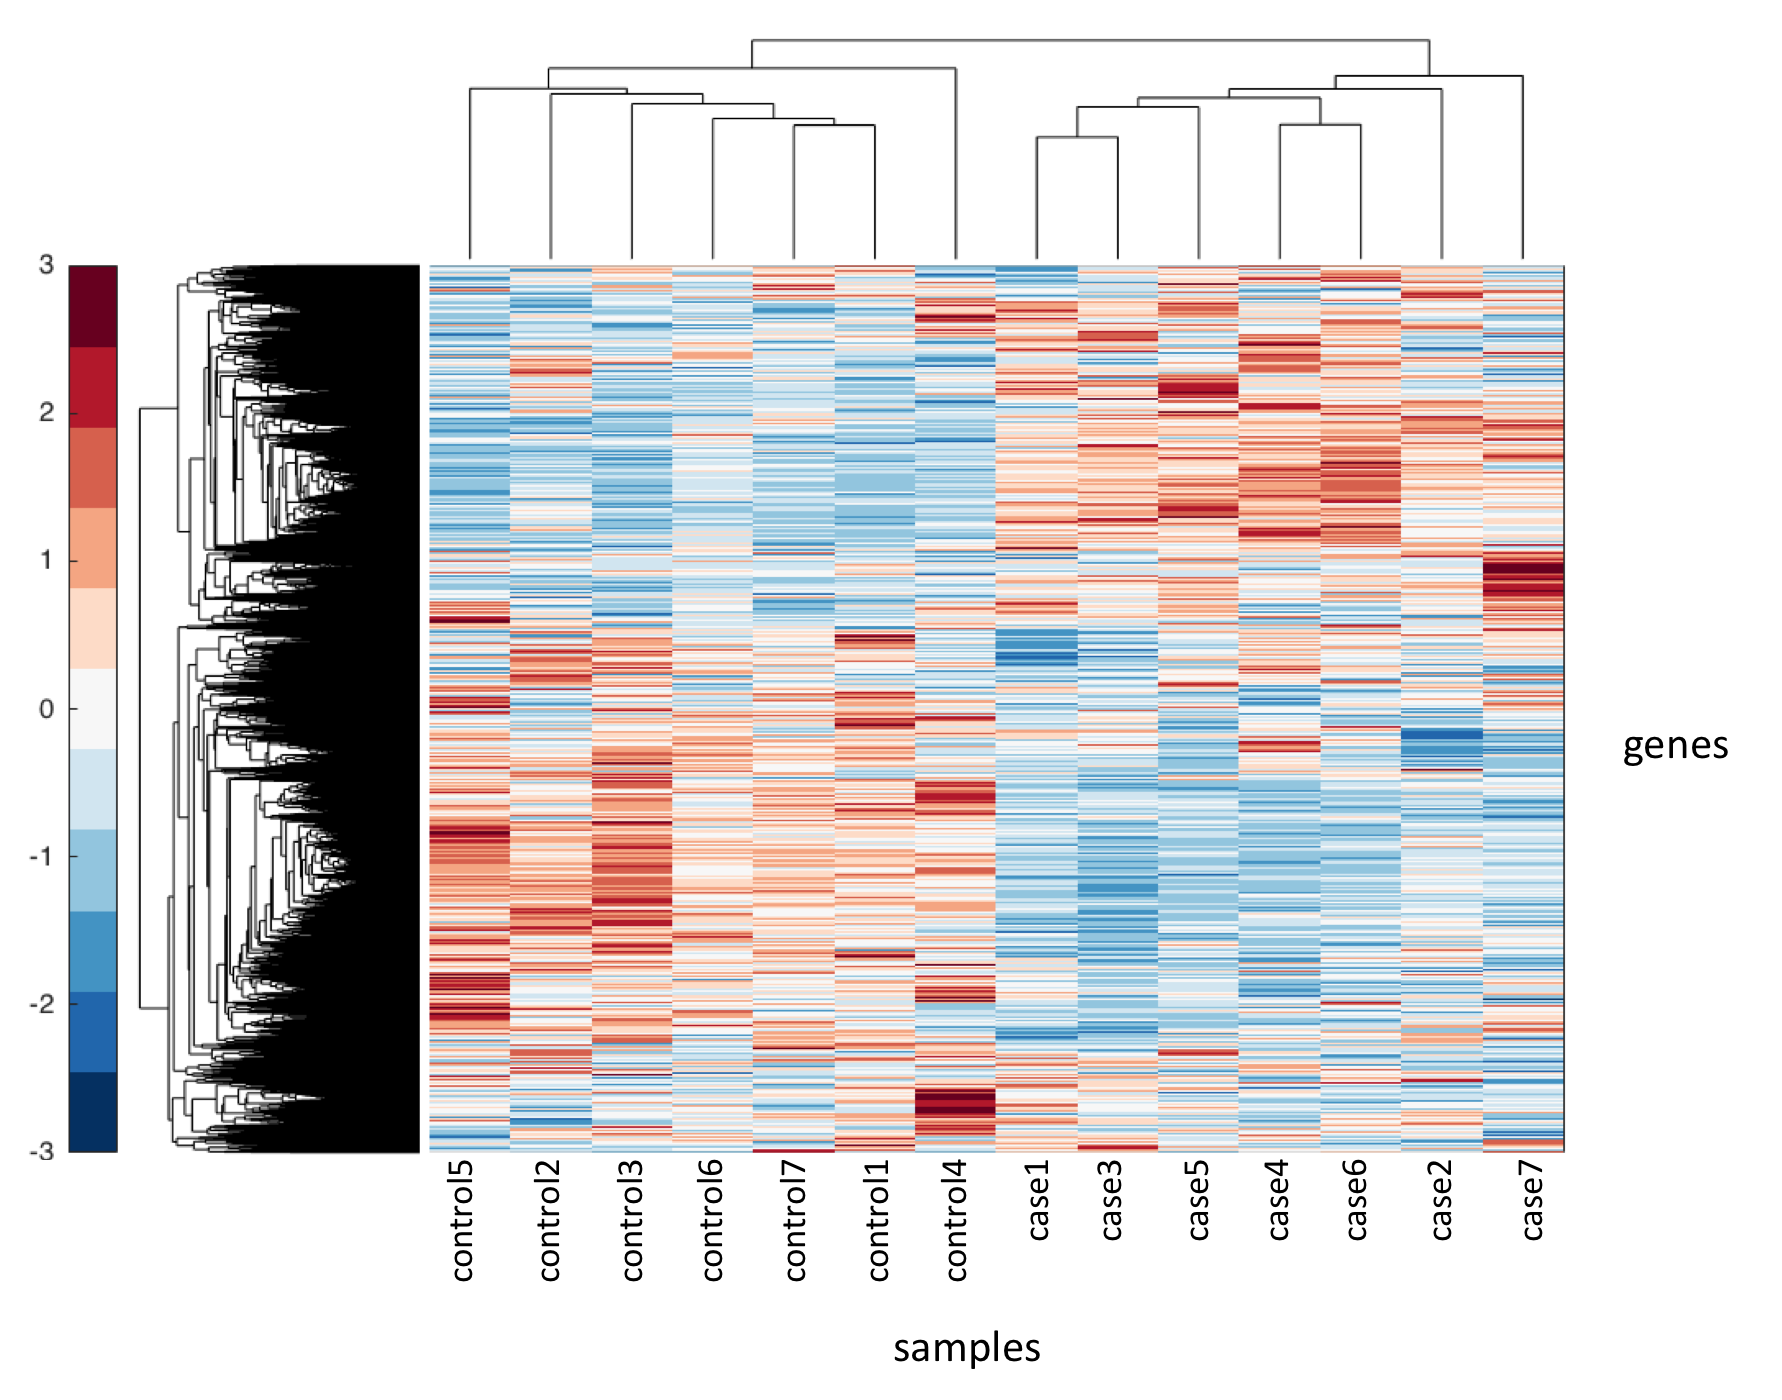
\includegraphics[width=\textwidth]{hierarchical-clustering}
	\caption{Example of hierarchical clustering using the MATLAB function clustergram}
	\label{fig:hierarchical-clustering}
\end{figure}


%Example of hierarchical clustering of simulated random numbers
%Figure: Example of clustergram of simulated random numbers
%No distinct clusters are observed. High and low expression values (red and blue colours) are mixed all together and the sample of the same type are mixed.



\subsubsection{Exercise: Hierarchical clustering for expression data}

Compute hierarchical clustering on the Fatty Liver \cite{Wruck2015}.
Since MATLAB is a commercial software, we will use a free to use wrapper for MATLAB's clustergram function. This wrapper is available from MultiPEN (\url{https://github.com/TGAC/MultiPEN/}, \cite{Rey2017}). The wrapper provided in MultiPEN reads the expression data provided as a tabular file and plots the hierarchical clustering image on screen, which is also saved as a png image. To use the wrapper just use MultiPEN in a terminal using the following syntax:

\paragraph{Syntax}
\paragraph{}

\begin{framed}
\begin{verbatim}
MultiPEN HierarchicalClustering Output Expression Threshold Title
\end{verbatim}
\end{framed}


\paragraph{Description}
\paragraph{}


{\bf MultiPEN}:  This is the path to the binary executable of MultiPEN

{\bf Output}:  Specify directory to save the output image, default is: {\it output/MultiPEN/stats/} 

{\bf Expression}: The expression data is in tabular format where the rows represent the features (e.g. genes) and the colums are the samples.

{\bf Threshold}: To filter expression values. For example, for gene expression, it is common practice to discard genes with counts smaller than 100. This is an optional input argument.

{\bf Title}: Specify the title to be displayed in the plot. This is an optional input argument.


%\begin{table}[!h]
%   \centering
%   %\caption{ }
%   \begin{tabulary}{\linewidth}{l L}
%      Parameter & Description \\
%      MultiPEN & This is the path to the binary executable of MultiPEN \\
%      Output & Specify directory to save the output image, default is: {\it output/MultiPEN/stats/} \\
%      Expression & The expression data is in tabular format where the rows represent the features (e.g. genes) and the colums are the samples. \\
%      Threshold & To filter expression values. For example, for gene expression, it is common practice to discard genes with counts smaller than 100. This is an optional input argument. \\
%      Title & Specify the title to be displayed in the plot. This is an optional input argument.
%   \label{tab:SyntaxisClustergram}
%   \end{tabulary}
%\end{table}

\paragraph{Exercise}
\paragraph{}

Run the the wrapper in MultiPEN to perform hierarchical clustering in the expression data for the Fatty Liver data \cite{Wruck2015} used in previous exercise. For more information on running MultiPEN visit \url{https://github.com/TGAC/MultiPEN/} \cite{Rey2017}.


\subsection{Interaction Network}
\subsubsection{Compile the network with Cytoscape}


\part{Part II}

\section{Statistical Approaches with Sparsity}

\subsection{Exercise: Features selection from expression data using MultiPEN}

Perform feature selection for the gene expression data on the Fatty Liver study \cite{Wruck2015}. Using the feature selection function provided by MultiPEN (\url{https://github.com/TGAC/MultiPEN/}, \cite{Rey2017}) which uses a penalised logistic regression approach. 

\paragraph{Syntax}
\paragraph{}

\begin{framed}
\begin{verbatim}
MultiPEN FeatureSelection Output Expression Interactions Class lambda 
DecisionThreshold NumIterations
\end{verbatim}
\end{framed}


\paragraph{Description}
\paragraph{}

{\bf MultiPEN}:  This is the path to the binary executable of MultiPEN

{\bf Output}:  Specify directory to save the output image, default is: {\it output/MultiPEN/stats/} 

{\bf Expression}: The expression data is in tabular format where the rows represent the features (e.g. genes) and the colums are the samples.

{\bf Interactions}: The interaction matrix where the i{\it th} interaction (row) is represented as: [source target score] where {\it source} and {\it target} are names (symbolID for genes and CHEBI IDs for metabolites) of the connected nodes and {\it score} is a number in the range [0,1] representing the interaction confidence (where 1 corresponds to the maximum level of confidence).

{\bf Class}: For each sample (one sample per row) specify if control (0) or case (1).

{\bf lambda}: This is the lambda parameter that optimises the logistic regression problem for your specific data. Different lambdas can be tested using cross validation, then selecting the value that provides better results (in terms of the size of the largest connected component, accuracy or area under the curve).  

{\bf DecisionThreshold}: The decision threshold is set to 0.5 by default. However, if want to test another value specify it here.

{\bf NumIterations}: Maximum number of iterations for the optimisation solver. Default value is 100.



\paragraph{Feature Selection Output Files}
\paragraph{}

Feature selection produces seven output files: 

\paragraph{}
{\bf MultiPEN-Rankings\_lambdaX.txt}: Ranking of features for the corresponding lambda X.

{\bf MultiPEN-Rankings\_lambdaX\_genes-higher-in-cases.txt}: Ranking of features which includes only features with higher expression in cases samples.

{\bf MultiPEN-Rankings\_lambdaX\_genes-higher-in-control.txt}: Ranking of features which includes only features with higher expression in control samples.

{\bf MultiPEN-vts\_lambdaX.txt}: Intercept term (logistic regression model).

{\bf MultiPEN-performance\_feature-selection\_lambdaX.txt}: file that contains statistics on the performance of feature selection: largest connected component (LCC), area under the curve (auc), accuracy, true positives (TP), true negatives (TN), false positives (FP) and false negatives (FN).

{\bf MultiPEN-feature-selection\_config.txt}: Contains the information of the parameters used: lambda, number of iterations and decision threshold.



%
%This tabular file contains the results for the features selection. The first five columns contain the list of features, weight, ranking, fold change and the class where the feature had higher vote.  The last columns correspond to the expression data. The columns are defined as follows:
%
%
%Column | Column Name | Description | Example (row 4 in Figure 2)
%-------|-------------|-------------|-----------------------------
%1 | name | Feature (gene and/or metabolite) name | PPOX
%2 | weight | This is the weight learned by MultiPEN and it is a number in the range [-1,1]. | 0.00290391
%3 | ranking | Ranking according to the absolute weight, where ranking 1 corresponds to the most significant feature for the model. | 3
%4 | foldChange | Fold change to determine the expression change from control to cases. | 1.1735
%5 | higherIn | The average expression is higher in case or control. | case
%6 | sample_1 | First sample | case1
%? | ? | ? | ?
%n+5 (n is the number of samples) | sample_n | Last sample | control7
%
%The figure shows an example of the rankings file created with the feature selection module.
%
%![example output rankings](images/example_output_rankings.png)
%
%
%**MultiPEN-Rankings_lambda0.001_genes-higher-in-cases.txt** and **MultiPEN-Rankings_lambda0.001_genes-higher-in-control.txt**
%
%These tabular files contain the ranking of features which includes only features with higher expression in cases samples and control samples separately. 
%
%
%**MultiPEN-vts_lambda0.001.txt**
%Intercept term (logistic regression model)
%
%
%MultiPEN-performance_feature-selection_lambda0.001.txt | LCC, auc, accuracy, TP, TN, FP, FN
%MultiPEN-feature-selection_config.txt | Lambda, number of iterations, decision threshold
%
%
%** MultiPEN-feature-selection_config.txt **
%File containing details of the parameters used to run feature selection: lambda, number of iterations (numIter - used to run the optimisation routine that solves the logistic regression problem) and the decision threshold (for class prediction). 
%
%
%
%### Example - OS
%
%*Using default decision threshold and number of iterations.*
%
%In the command line, navigate to the folder where the binary for MultiPEN is located, i.e., binary-OS/MultiPEN_v001_OS/. Then create variables for the paths to stand-alone application, output directory and input files by typing:
%
%```
%MultiPEN="MultiPEN.app/Contents/MacOS/applauncher"
%OutputDirectory="ExampleOutputs/"
%ExpressionData="ExampleInputs/X.txt"
%Interactions="ExampleInputs/E.txt"
%SampleClass="ExampleInputs/Y.txt"
%lambda=0.001
%```
%
%
%Next, run feature selection with the following command:
%
%```
%$MultiPEN FeatureSelection $OutputDirectory $ExpressionData $Interactions $SampleClass $lambda
%```
%
%
%### Running example script for feature selection
%
%To run the script provided as example with all the default parameters, use the command:
%
%```
%./example_feature_selection.sh 
%```





\section{Pathway Analysis}

Objective

Steps

Input data
A list of ranked genes. For this session we will use the rankings from feature selection in ExampleOutputs\/MultiPEN\-Rankings\_lambda0.0001.txt.

To run the R script type in the terminal:

Rscript enrichmentGO.R ../ExampleOutputs/MultiPEN\-Rankings\_lambda0.0001.txt output/




% Boxed code
%\begin{framed}
%\begin{verbatim}
%	
%\end{verbatim}
%\end{framed}


%Example to create a list
%List:
%\begin{itemize}
%	\item item 1
%	\item item 2		
%\end{itemize}


%Example to enumerate a list
%\begin{enumerate}	
%	\item enumerated item
%	\item another item
%\end{enumerate}


%Figure resference \autoref{fig:volcanoplot}). 
%
%\begin{figure}[!h]
%	\centering
%	\includegraphics[width=\textwidth]{VolcanoMatrix}
%	\caption{Matrix of volcano plots explore genes that differ significantly between pairs of conditions}
%	\label{fig:volcanoplot}
%\end{figure}

%figure with subfigures
%\begin{figure}[!h]
%	\centering
%	\begin{subfigure}{.3\textwidth}
%		\includegraphics[width=\textwidth]{MAPlotEPS1_8_EPS2_8}
%		\caption{MA for EPS1 and EPS2, 8 hours}
%		\label{fig:MAPlotEPS1_8_EPS2_8}
%	\end{subfigure}
%	\begin{subfigure}{0.3\textwidth}
%		\includegraphics[width=\textwidth]{MAPlotEPS1_8_noEPS_8}
%		\caption{MA for EPS1 and noEPS, 8 hours}
%		\label{fig:MAPlotEPS1_8_noEPS_8}
%	\end{subfigure}
%	\begin{subfigure}{.3\textwidth}
%		\includegraphics[width=\textwidth]{MAPlotEPS2_8_noEPS_8}
%		\caption{MA for EPS2 and noEPS, 8 hours}
%		\label{fig:MAPlotEPS2_8_noEPS_8}
%	\end{subfigure}
%	\caption{Average intensity vs log ratio Plots, for 8 hours}
%	\label{fig:MAPlot_8hours}
%\end{figure}


%See below example of table  \autoref{tab:table1}
%\begin{table}[h]
%	\centering
%	\caption{Example of table 1}
%	\begin{tabular}{c | c | c}
%		\hline
%		column 1 & column 2 & column 3 \\
%		\hline
%		aaaaa  & bbbbbbb & ccccccc \\ 
%		xxxxxxx  & yyyyyyyy & zzzzzzzz \\		
%		\label{tab:table1}
%	\end{tabular}
%\end{table}





\bibliography{references}
\bibliographystyle{plain}

\end{document}  